%!TEX root = ../Report.tex
\section{Assumptions} % (fold)
\label{sec:assumptions}

	\subsection{Target Audience} % (fold)
	\label{sub:target_audience}
	The major target audience would be the people pursuing post-graduate studies or professionals interested in practical and applicable skills in the industry.

	Current NUS-ISS students can also enjoy the benefit if they want to get the quick enquiry reply.
	% subsection target_audience (end)

	\subsection{Data Quality} % (fold)
	\label{sub:data_quality}
	All information used to build IChat is from NUS-ISS website \cite{nusiss}. It is assumed the data provided by NUS-ISS website are correct.
	% subsection data_quality (end)

% section assumptions (end)

\section{Project Scope} % (fold)
\label{sec:project_scope}
	In this project, a chatbot system (IChat) based on NUS-ISS website data is performed via Dialogflow \cite{dialogflow}. IChat focuses on two parts: \textbf{(i)} \textbf{intent-based system} \cite{intentsoverview}; \textbf{(ii)} \textbf{knowledge-based system} \cite{knowledgeconnector}. The inquires related to Graduate Programmes are replied by the former system while the inquiries related to the courses of Executive Education Programmes and Stackable Certificate Programmes are answered by the knowledge-based system.

	The intent-based system can answer question with context \cite{context} via \textbf{rich messages response} \cite{richmessage} option or manual input. It includes questions related to Admission \& Application, Career Path, Fee \& Loans, Modules, Overview and Project \& Internship for each Graduate Programme.

	The knowledge-based system can only answer questions for over 130 courses listed in Executive Education Flyer \cite{course}. It covers Course Overview, Key Takeaway, Target Audience, Prerequisites, Course Details, Fees \& Loans and Certification.
% section project_scope (end)

\section{Knowledge Model} % (fold)
\label{sec:knowledge_model}
	Knowledge modeling can be classified into three parts \cite{schreiber2001knowledge}:
	\begin{enumerate}[label=(\roman*)]
		\item Knowledge identification
		\item Knowledge specification
		\item Knowledge refinement
	\end{enumerate}

	\subsection{Knowledge Identification} % (fold)
	\label{sub:knowledge_identification}
		Knowledge identification sets the groundwork for the next stage encompassing knowledge specification. Information sources that are deemed to be useful are identified in preparation of knowledge acquisitions. In the context of building a chatbot, two main sources have been identified and are documented in Table \ref{table:knowledgesource}.

		\begin{table}[h]
		\centering
		\resizebox{\textwidth}{!}{%
		\begin{tabular}{|l|p{3cm}|p{5cm}|p{7cm}|}
		\hline
		\textbf{S/N} & \textbf{Source of Information} & \textbf{Insights from information sources} & \textbf{Knowledge acquisition technique} \\ \hline
		\textbf{1} & NUS ISS website & It provides basic information on different postgraduate programs & Data gathering from publicly available/documented information \\ \hline
		\textbf{2} & Generic Population & To validate and support the assumptions & Elicitation of tacit knowledge through analysis result of feedback from general population \\ \hline
		\end{tabular}%
		}
		\caption{Knowledge Source and Acquisition Technique}
		\label{table:knowledgesource}
		\end{table}
	% subsection knowledge_identification (end)

	\subsection{Knowledge Acquisition} % (fold)
	\label{sub:knowledge_acquisition}
		Following from the identification of knowledge sources, knowledge acquisition is conducted to capture the problem-solving domain knowledge. The techniques adopted to acquire the knowledge have been describe in Table \ref{table:knowledgesource} and the corresponding results are presented using a dependency diagram as shown in Figure \ref{fig:knowledge_model}.

		\begin{figure}[h]
			\centering
			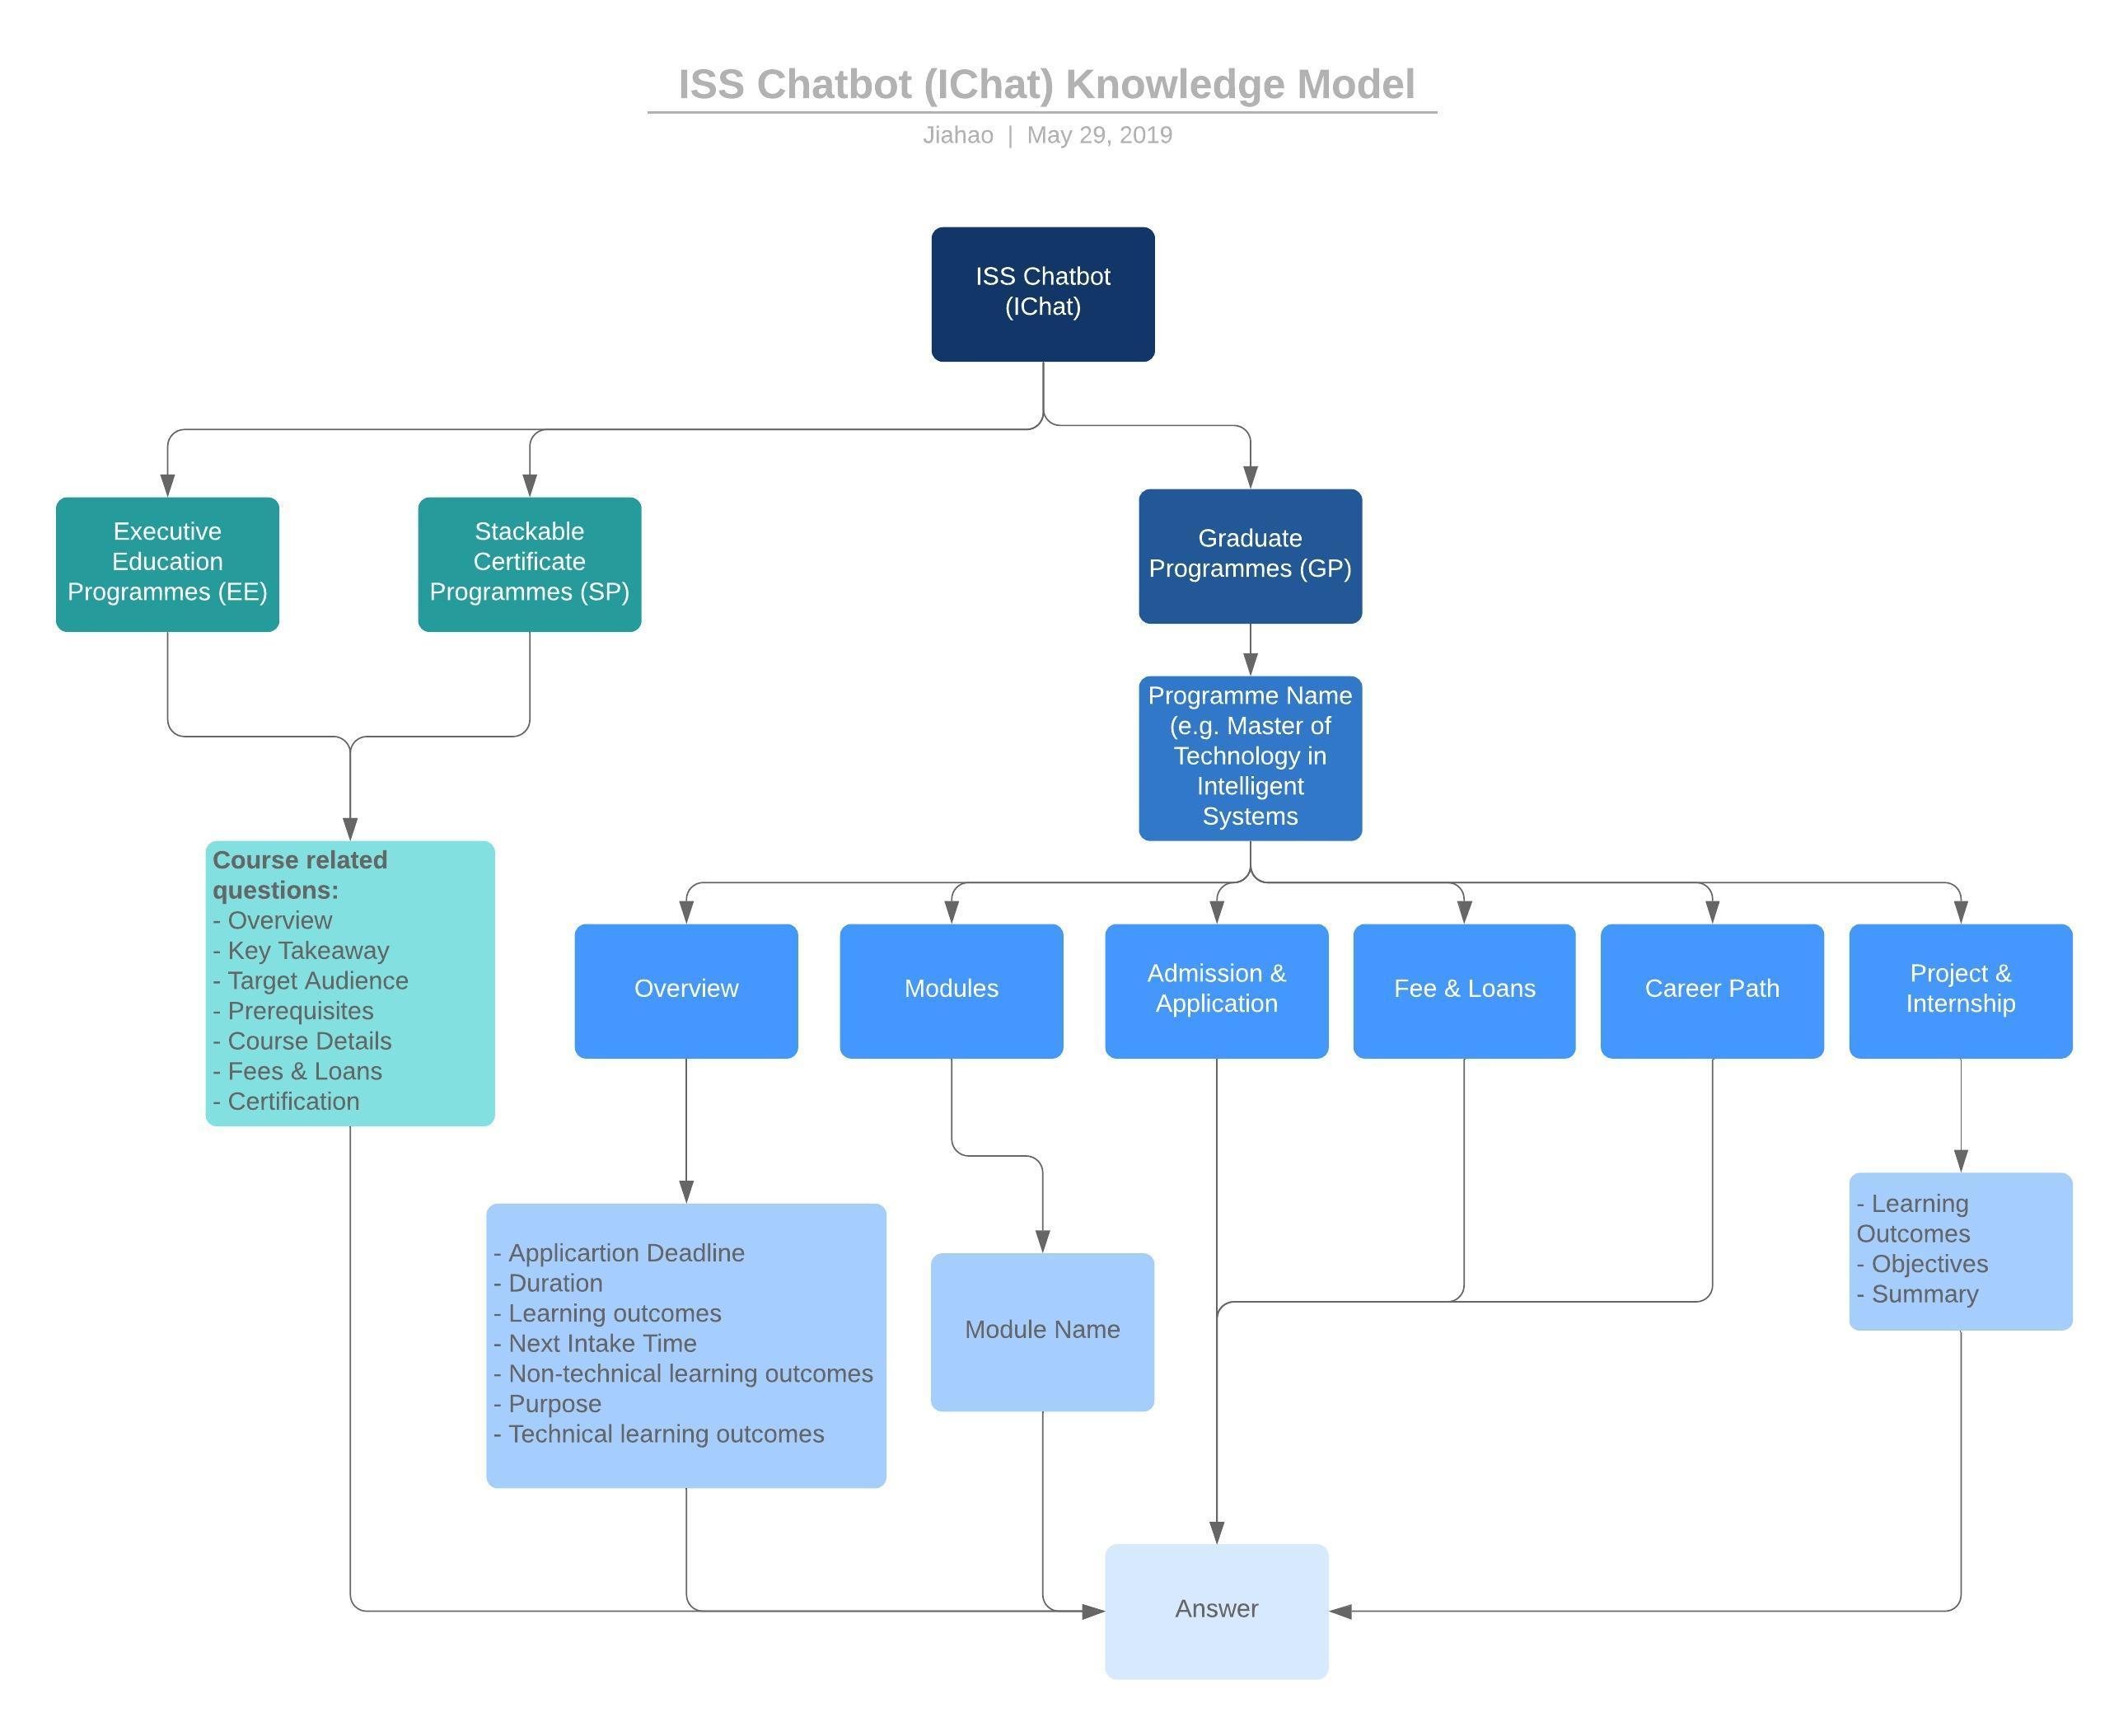
\includegraphics[width=\linewidth]{img/knowledge_model.jpeg}
			\caption{Domain Model of IChat}
			\label{fig:knowledge_model}
		\end{figure}

		The domain diagram arranges the factors affecting user’s question flow in a hierarchical tree structure. The top most level node represents the description of the proposed chatbot, which in this case, called iChat chatbot for NUS ISS website pages. This chatbot can be broken down into multiple layers of different components before arriving at the answers. These question flows are gathered from users of proposed question flow and represent their inherent preference. Table \ref{table:exampe_depedency} illustrates an example using the composition tree diagram in \ref{fig:knowledge_model}.

		The second level nodes represent the program we focused for the chatbot system and as well as the following detailed level nodes for more specific areas that may be asked within the chatbot system.

		\begin{table}[]
		\centering
		\resizebox{\textwidth}{!}{%
		\begin{tabular}{|l|p{4cm}|p{9cm}|}
			\hline
			S/N & \textbf{Category} & \textbf{Information} \\ \hline
			\textbf{1} & Observable & A user who is keen to explore postgraduate program in NUS-ISS \\ \hline
			\textbf{2} & Inferable sub-goals & The user in “1” might be interested in a master program. He/she might also be only eligible for a given subset of master program \\ \hline
			\textbf{3} & Top-level inference & The sub-goal in “2” is also one of the main factors that affects a user’s choice of a suitable master program \\ \hline
		\end{tabular}%
		}
		\caption{Example to Show A Part of the Dependency Diagram}
		\label{table:exampe_depedency}
		\end{table}
	% subsection knowledge_acquisition (end)

	\subsection{Knowledge Refinement} % (fold)
	\label{sub:knowledge_refinement}
		The knowledge refinement is an iterative process and it include model validation and model refinement. For model validation, different sets of test data will be used to run the simulation, and the result will be compared with sample data.

		For model refinement, after getting different actual results from expected results, we adjust the training phrases into different formats and retest it with the confidence score again to modify the model.
	% subsection knowledge_refinement (end)

% section knowledge_model (end)

\section{System Architecture} % (fold)
\label{sec:system_architecture}

	\begin{figure}[h]
		\centering
		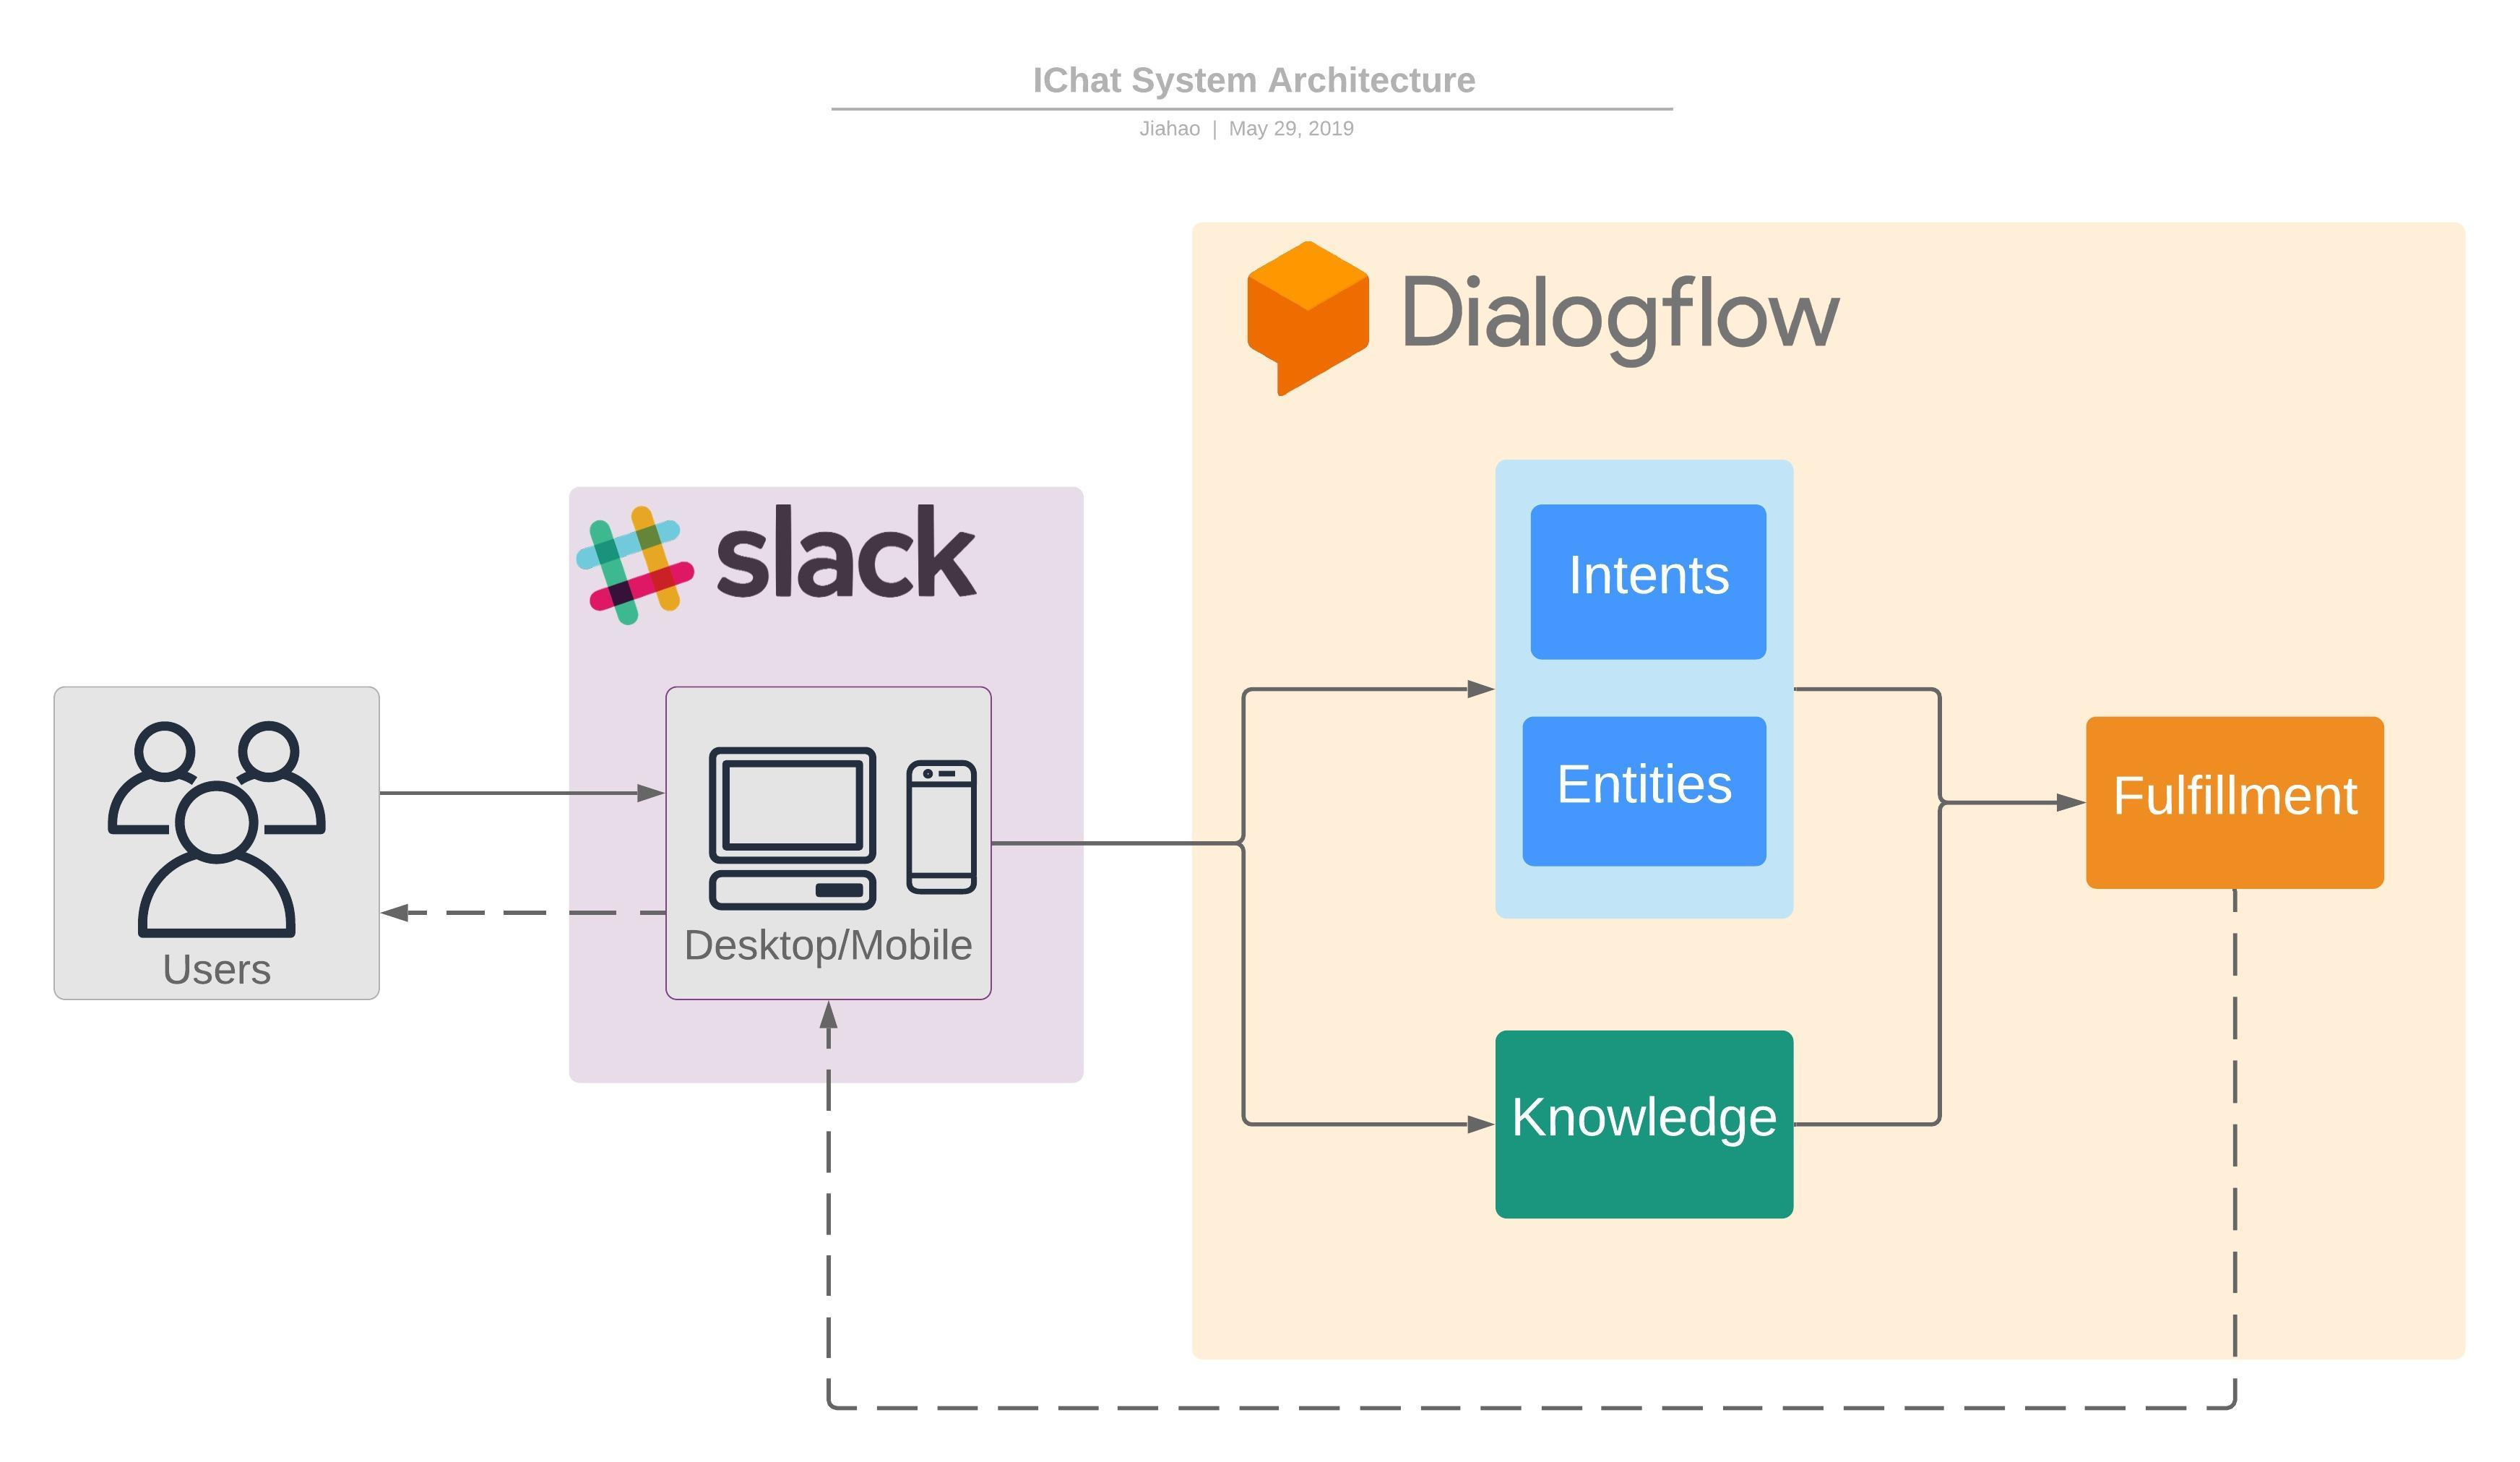
\includegraphics[width=\linewidth]{img/system_architecture.jpeg}
		\caption{System Architecture Diagram}
		\label{fig:system_architecture_diagram}
	\end{figure}
	Figure \ref{fig:system_architecture_diagram} shows the system architecture diagram of IChat. It illustrates how the different components interact with each other through Dialogflow. After the user keys in the inputs in the Slack by either mobile phone or computer, Slack will be passed the input through the Dialogflow to process. Based on the enquiries from the user, Dialogflow will choose either intent-based system or knowledge-based system to answer. Then the data will be passed to fulfillment and return the results to Slack so the user can read the answer.
% section system_architecture (end)